\chapter{Support Vector Machine}\label{chap:SVC}
In questo capitolo si descrive genericamente la famiglia dei modelli \emph{support vector machine} (SVM) e in dettaglio la formulazione del modello per risolvere problemi di classificazione (\emph{support vector classifier}, o SVC). 
Nel~\Cref{sec:kernel_methods} si fornisce una breve introduzione ai metodi \emph{kernel} e alla famiglia dei modelli SVM. 
Nel~\Cref{sec:hard_margin_classifier} si descrive la formulazione \emph{hard margin} per problemi di classificazione, che non ammette dati erroneamente etichettati.
Nel~\Cref{sec:soft_margin_classifier} si descrive la formulazione \emph{soft margin} per problemi di classificazione, che ammette la presenza di dati erroneamente etichettati.
Nel~\Cref{sec:kernel_trick} si descrive l'utilizzo del metodo \emph{kernel} per i modelli SVC.
Per concludere, nel~\Cref{sec:svc_limiti} si descrivono in generale le principali limitazioni dei modelli SVM.

\section{Metodi kernel}\label{sec:kernel_methods}
\`E possibile suddividere i modelli di apprendimento automatico in due categorie: modelli lineari e modelli non lineari. 
I modelli lineari vengono utilizzati nei casi in cui si assume che la relazione tra i dati di addestramento $\Vec{x}$ e le etichette $y$ possa essere approssimata in modo accettabile da una funzione lineare $f(\Vec{x}) = \Vec{w}\cdot\Vec{x} + b$, mentre i modelli non lineari sono in grado di approssimare relazioni più complesse.
%I modelli non lineari vengono utilizzati nei casi in cui questa assunzione non si dimostra vera, e per cui serve definire una funzione più complessa per approssimare la relazione.
In genere, produrre un modello lineare è relativamente facile, ma molti scenari reali esprimono relazioni non lineari. 
Adottare un modello lineare in questi casi porterebbe ad insufficienti capacità di generalizzazione, dovute alla troppa semplicità del modello (\emph{underfitting}). 
\`E quindi necessario sviluppare algoritmi per produrre modelli in grado di esprimere relazioni non lineari, ma utilizzare un modello più complesso potrebbe comunque portare ad insufficienti capacità di generalizzazione. 
Questo problema si potrebbe verificare nel caso in cui il modello si adatti troppo fedelmente ai dati di addestramento (\emph{overfitting}).
Questa problematica è descritta nel~\Cref{sec:bias_variance_tradeoff}; mentre in~\Cref{fig:esempio_underfitting_overfitting} si mostrano esempi di \emph{underfitting} o \emph{overfitting}.

Si vorrebbe quindi un modello sufficientemente complesso per approssimare la relazione espressa dai dati, ma allo stesso tempo non troppo complesso da soffrire di \emph{overfitting}; si vorrebbe la semplicità di un modello lineare con le capacità di modellazione di un modello non lineare. 
% TODO: potrebbe benissimo andare nel capitolo 1
\begin{figure}
    \begin{subfigure}[t]{.45\textwidth}
        \centering
        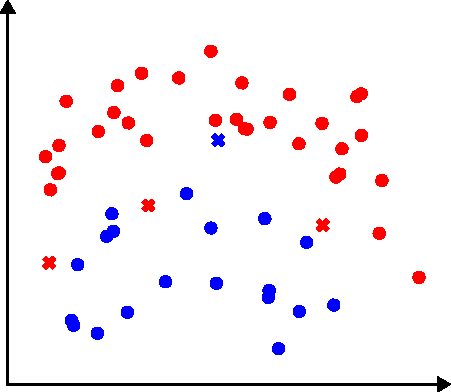
\includegraphics[width=\textwidth]{img/under_over_fitting_1.pdf}
        \caption{Il colore identifica la classe; i punti scorrettamente etichettati sono indicati con il simbolo x.}
    \end{subfigure}%
    \hfill
    \begin{subfigure}[t]{.45\textwidth}
        \centering
        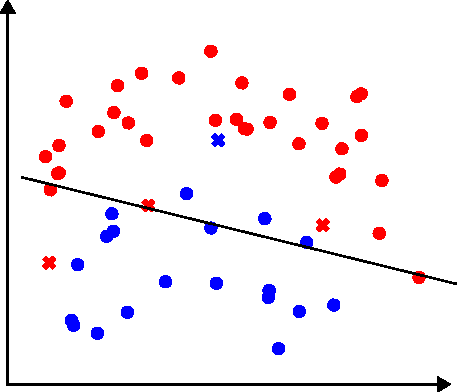
\includegraphics[width=\textwidth]{img/under_over_fitting_2.pdf}
        \caption{Esempio di come un modello lineare potrebbe esibire \emph{underfitting}.}
    \end{subfigure}%
\vskip\baselineskip
    \begin{subfigure}[t]{.45\textwidth}
        \centering
        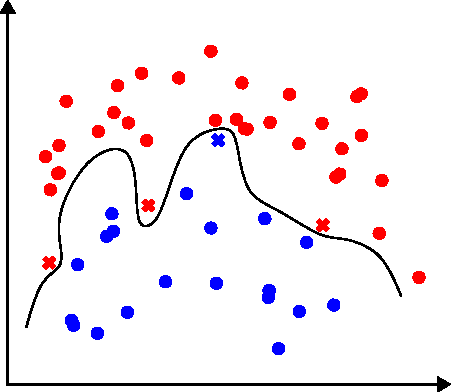
\includegraphics[width=\textwidth]{img/under_over_fitting_3.pdf}
        \caption{Esempio di come un modello non lineare potrebbe esibire \emph{overfitting}.}
    \end{subfigure}%
    \hfill
    \begin{subfigure}[t]{.45\textwidth}
        \centering
        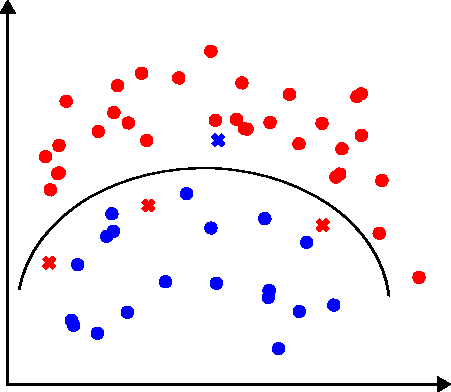
\includegraphics[width=\textwidth]{img/under_over_fitting_4.pdf}
        \caption{Esempio di una possibile superficie di separazione con buone capacità di generalizzazione.}
    \end{subfigure}%
\caption{Esempio di \emph{underfitting} e \emph{overfitting} su un dataset per un problema di classificazione binaria.}
\label{fig:esempio_underfitting_overfitting}
\end{figure}

I \emph{metodi kernel}\cite{2007_kernel_methods} sono una famiglia di approcci per risolvere vari problemi tipici dell'apprendimento automatico. La particolarità sta nel fatto che non si tratta di metodi creati \emph{ad hoc}, ma di estensioni di algoritmi lineari già noti, potenziati per poter esprimere relazioni più complesse.
L'idea alla base dei metodi \emph{kernel} è di mappare i dati dallo spazio originale $\mathcal{X}$ ad un nuovo spazio $\mathcal{H}$, chiamato \emph{spazio delle feature}, di dimensionalità maggiore rispetto ad $\mathcal{X}$, potenzialmente infinita, utilizzando la trasformazione non lineare $\Phi: \mathcal{X} \rightarrow \mathcal{H}$.
Nello spazio delle \emph{feature} i dati diventano linearmente separabili, ed è quindi possibile utilizzare un modello lineare espresso esclusivamente in termini di prodotto scalare tra elementi in $\mathcal{H}$, ma che esprime una relazione non lineare in $\mathcal{X}$.

Questo procedimento è però costoso dal punto di vista computazionale: va calcolata $\Phi$ per ogni punto e poi va calcolato il prodotto interno tra tutte le coppie di elementi.
I metodi \emph{kernel} evitano di utilizzare esplicitamente la funzione $\Phi$, utilizzando invece una funzione
%Nei metodi \emph{kernel} lo spazio delle \emph{feature} è un \emph{reproducing kernel Hilbert space} (RKHS) \cite{}: questo consente di esprimere il prodotto scalare tra elementi appartenenti ad $\mathcal{H}$ con una funzione espressa in termini di prodotto scalare tra elementi di $\mathcal{X}$. Esiste quindi la funzione 
\begin{equation*}
    K: \mathcal{X} \times \mathcal{X} \rightarrow \mathbb{R} 
\end{equation*}
per cui per ogni $\Vec{x}, \Vec{z} \in \mathcal{X}$ vale
\begin{equation*}
    K(\Vec{x}, \Vec{z}) = \Phi(\Vec{x}) \cdot \Phi(\Vec{z}).
\end{equation*}
Questa funzione $K$ è chiamata \emph{funzione kernel}.
Un metodo \emph{kernel} è un algoritmo di addestramento che riesce a sfruttare una funzione \emph{kernel} nelle fasi di addestramento e predizione, rendendo in questo modo non necessario l'utilizzo di $\Phi$, perché il prodotto scalare delle immagini $\Phi(\Vec{x}) \cdot \Phi(\Vec{z})$ è funzione del prodotto scalare tra $\Vec{x}, \Vec{z}$ nello spazio originale.
Questo calcolo è possibile perché $\mathcal{H}$ è un \emph{reproducing kernel Hilbert space}(RKHS)~\cite{RKHS}.

Con un metodo \emph{kernel} si cerca di sfruttare la semplicità di un modello lineare nello spazio delle \emph{feature} ma in grado di modellare relazioni complesse nello spazio originale.
Il~\Cref{sec:kernel_trick} riporta una spiegazione più approfondita dell'applicazione del metodo \emph{kernel} ai modelli SVC.

Tra i metodi \emph{kernel} più noti possiamo citare \emph{kernel principal component analysis}\cite{kernel_PCA} o \emph{kernel perceptron}\cite{kernel_perceptron}, ma l'approccio forse più importante è quello relativo alla famiglia delle \emph{support vector machine}, che include varianti per risolvere sia problemi di classificazione che di regressione.
Introdotti inizialmente per problemi di classificazione, i modelli SVC estendono il concetto di \emph{maximal margin classifier}. 
L'addestramento di un modello SVC ha come obiettivo quello di trovare un iperpiano che separa i punti appartenenti a due classi diverse con il massimo margine di separazione ottenibile. 
Questo approccio era inizialmente limitato a problemi lineari senza ammissione di dati erroneamente etichettati. 
Nei primi anni novanta, con l'introduzione del metodo \emph{kernel}\cite{1992_hardmargin_svm} prima e con l'introduzione della formulazione \emph{soft margin}\cite{1995_svm} poi, i modelli SVC divennero delle buone opzioni per risolvere problemi di classificazione non lineari e con dati erroneamente etichettati, riscuotendo un buon successo e ottenendo in alcuni casi \emph{performance} comparabili e spesso superiori ad altri modelli avanzati. 

Si trovano in letteratura diversi approcci che modificano la formulazione SVM originale, come per esempio \emph{$\nu$-svm}\cite{2000_nu_svm} o  \emph{p-svm}\cite{2001_p_svm}.
In questa tesi si presterà particolare attenzione alla formulazione originale per risolvere problemi di classificazione, dato che è la formulazione di partenza considerata per l'approccio proposto nel~\Cref{sec:our_budgeted_svm}.

Le formulazioni dei modelli SVC esposte nei prossimi paragrafi sono estratte in gran parte da~\cite{1995_svm,svm_tutorial,elements-of-statistical-learning}.

\section{Classificazione \emph{hard margin}}\label{sec:hard_margin_classifier}
Si ipotizza di avere un insieme di dati $\mathcal{X} = \{\Vec{x}_i, i=1,\dots,m\}$ contenente $m$ vettori $d$-dimensionali, ovvero $\Vec{x}_i \in \mathbb{R}^d$. 
Ogni $\Vec{x}_i$ ha associata un etichetta $y_i \in \{-1, +1\}$: si considerano quindi problemi di classificazione binaria.
%
L'insieme $\mathcal{X}$ è linearmente separabile se esistono un vettore $\Vec{w} \in \mathbb{R}^d$ e uno scalare $b \in \mathbb{R}$ (chiamato \emph{bias}) che identificano un iperpiano $\Vec{w}\cdot \Vec{x} +b=0$ in grado di separare perfettamente le due classi di dati.
\begin{figure}
    \centering
    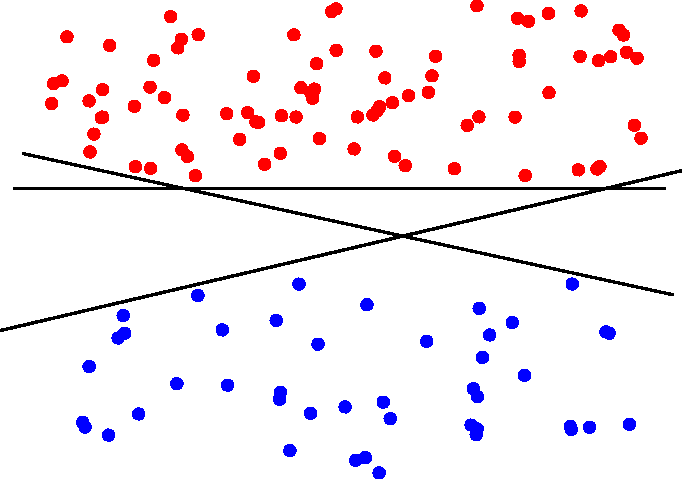
\includegraphics[width=0.5\linewidth]{img/dati_linearmente_separabili.pdf}
    \caption{Esempio di dati per un problema di classificazione binaria in cui le classi (identificate dai due colori rosso e blu) sono linearmente separabili. Sono illustrate alcune delle possibili rette in grado di separare correttamente tutti gli esempi della stessa classe. }
    \label{fig:dati_linearmente_separabili}
\end{figure}
Con $\Vec{w}$ e $b$ noti, si definisce il classificatore 
\begin{equation*}
    h(\Vec{x}) = \sign(\Vec{w}\cdot \Vec{x} +b).
\end{equation*} 
Per insiemi di dati linearmente separabili esistono infiniti iperpiani che li separano; l'interesse è di trovare un iperpiano con cui eseguire predizioni accurate su nuovi dati. 
Si riporta in~\Cref{fig:dati_linearmente_separabili} un esempio di insieme di dati con alcuni possibili superfici di separazione. 
Per costruire un buon classificatore, in grado di generalizzare su dati mai visti nella procedura di addestramento, si vorrebbe identificare l'iperpiano che massimizza il margine di separazione tra le due classi, ovvero l'iperpiano che massimizza la distanza tra l'iperpiano stesso e i punti più vicini di ogni classe.
La superficie di separazione deve essere equidistante rispetto agli esempi più vicini di ogni classe.

Per configurare un problema trattabile è necessario quantificare il margine.
Sia $d$ la distanza tra la superficie di separazione e il punto più vicino etichettato come positivo. 
Dato che si vorrebbero separare al meglio le due classi, la superficie di separazione dovrà trovarsi alla stessa distanza anche rispetto al punto più vicino etichettato come negativo.
In~\Cref{fig:optimal_separation_margin} si può vedere un esempio per un insieme di dati in due dimensioni.
Il margine è quindi $M=2d$, ma è possibile trasformarlo in una forma più conveniente.
Si definiscono a tale scopo i vincoli 
\begin{equation*}\label{eq:svc:hardmargin:margin_1}
    \Vec{w}\Vec{x}_i + b \geq 1 \quad \text{se} \quad y_i = +1 \quad  i=1,\dots,m,
\end{equation*}
\begin{equation*}
    \Vec{w}\Vec{x}_i + b \leq -1 \quad \text{se} \quad y_i = -1 \quad i=1,\dots,m,
\end{equation*}
che forzano la superficie di separazione ad essere equidistante dagli iperpiani su cui giacciono i punti più vicini di ogni classe.
% Dividendo entrambi i lati delle disequazioni per $M$
% \begin{equation*}
% \frac{1}{M}\Vec{w}\Vec{x}_i + \frac{1}{M}b \geq 1,
% \end{equation*}
% \begin{equation*}
% \frac{1}{M}\Vec{w}\Vec{x}_i + \frac{1}{M}b \leq -1,
% \end{equation*}
% otteniamo come iperpiano di classificazione $\frac{1}{M}\Vec{w}\Vec{x}_i + \frac{1}{M}b = 0,$ che è equivalente a $\Vec{w}\Vec{x}_i + b = 0$. Il parametro $M$ è quindi in genere fissato ad $1$.
Dato che $y_i\in\{-1,1\}$, i vincoli precedenti possono essere combinati in
\begin{equation*}
    y_i(\Vec{w}\Vec{x}_i + b) \geq 1 \quad i=1, ..., m.
\end{equation*}
Considerando i punti per cui il vincolo precedente è un uguaglianza: i punti positivi saranno sull'iperpiano $H1: \vec{w}\cdot \vec{x} + b=+1$, con vettore normale $\vec{w}$ e distanza dall'origine $|1-b|/\norm{\vec{w}}$, mentre i punti negativi saranno sull'iperpiano $H2: \vec{w}\cdot \vec{x} + b=-1$, con vettore normale $\vec{w}$ e distanza dall'origine $|-1-b|/\norm{\vec{w}}$. Si può dimostrare che la distanza $2d$ è equivalente a $2/\norm{\vec{w}}$~\cite{svm_tutorial}.

L'iperpiano ottimo $H0: \Vec{w}^*\Vec{x} + b^* = 0$ è l'iperpiano che separa linearmente $\mathcal{X}$ massimizzando il margine di separazione; il simbolo $*$ indica il valore ottimo di una variabile.

I punti $\Vec{x}_i$ per cui $\Vec{w}^*\Vec{x}_i + b^* = \pm 1$ sono chiamati \emph{vettori di supporto}.
\begin{figure}
    \centering
    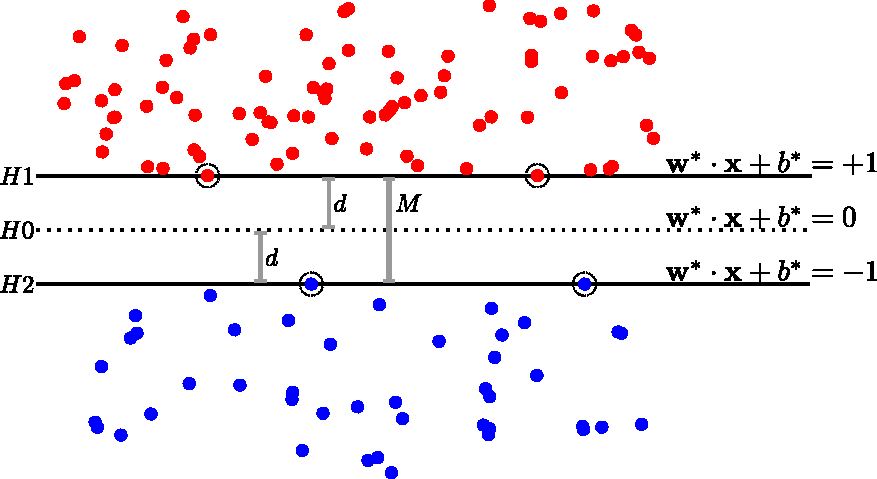
\includegraphics[width=0.7\linewidth]{img/margine_separazione.pdf}
    \caption{Esempio di superficie di separazione con margine massimale per gli stessi dati utilizzati in~\Cref{fig:dati_linearmente_separabili}. I punti cerchiati sono vettori di supporto. $H0$ è la superficie di separazione, mentre $H1$ e $H2$ sono le superfici su cui giacciono i vettori di supporto. Il margine è $M=2d$.}
    \label{fig:optimal_separation_margin}
\end{figure}
%
Massimizzare il margine $2/\norm{\vec{w}}$ equivale a minimizzare $\norm{\Vec{w}}$. 
Trovare la superficie di separazione con margine massimale equivale quindi a risolvere il problema di ottimizzazione
\begin{equation}
\label{eq:svc:hardmargin:primal}
\begin{aligned}
& \min_{\Vec{w},b} && \norm{\Vec{w}} \\
& \textrm{s.t.} && y_i(\Vec{w}\cdot \Vec{x}_i + b) \geq 1, && i=1,\dots,m. \\
\end{aligned}
\end{equation}
Questo problema ha funzione obiettivo quadratica e vincoli lineari.
Viene tradizionalmente risolto considerando una formulazione duale.

\subsection{Formulazione duale}\label{subsec:hard_margin_dual}
Si riscrive la funzione obiettivo del problema primale in~\Cref{eq:svc:hardmargin:primal} in una forma più conveniente e si esprimono i vincoli in forma normale, ottenendo il problema
\begin{equation}\label{eq:svc:hardmargin:primal_convenient}
\begin{aligned}
& \min_{\Vec{w},b}    && \frac{1}{2}\norm{\Vec{w}}^2 \\
& \textrm{s.t.} && y_i(\Vec{w}\cdot \Vec{x}_i + b) - 1 \geq 0, && i=1,\dots,m. \\
\end{aligned}
\end{equation}
%
Applicando il metodo dei moltiplicatori di Lagrange~\cite{optimization_book} si ottiene la funzione lagrangiana
\begin{equation}
\label{eq:svc:hardmargin:lagrangian}
\begin{split}
L_P(\Vec{w},b, \vec{\alpha})  & = \frac{1}{2}\norm{\Vec{w}}^2 - \sum_{i=1}^{m} \alpha_i (y_i(\Vec{w}\cdot \Vec{x}_i +b) -1) =\\
        & = \frac{1}{2}\Vec{w} \cdot \Vec{w} - \sum_{i=1}^{m} \alpha_i y_i(\Vec{w}\cdot \Vec{x}_i +b) -  \sum_{i=1}^{m} - \alpha_i = \\
        & = \frac{1}{2}\Vec{w}\cdot\Vec{w} - \sum_{i=1}^{m} \alpha_i y_i \Vec{w}\cdot \Vec{x}_i - b \sum_{i=1}^{m} \alpha_i y_i + \sum_{i=1}^{m} \alpha_i,
\end{split}
\end{equation}
da minimizzare rispetto a $\Vec{w},b$ e da massimizzare rispetto ad $\Vec{\alpha}$ 
\begin{equation}
\label{eq:svc:hardmargin:max_min}
\begin{aligned}
& \max_{\vec{\alpha}} \min_{\Vec{w}, b} && L_P(\Vec{w},b, \Vec{\alpha}) \\
& \textrm{s.t.} && \alpha_i \geq 0, && i=1,..., m.\\
\end{aligned}
\end{equation}
%
%
Una soluzione ottima per il problema~\Cref{eq:svc:hardmargin:max_min} deve soddisfare le condizioni di Karush-Kuhn-Tucker (KKT)\cite{svm_tutorial,optimization_book}:
\begin{align}
    \label{eq:svc:hardmargin:kkt1}
    \pd{L_P(\Vec{w},b,\vec{\alpha})}{\Vec{w}} = \Vec{0}, \\[2mm]
    \label{eq:svc:hardmargin:kkt2}
    \pd{L_P(\Vec{w},b,\vec{\alpha})}{b} = 0, 
\end{align}
\begin{align}
    \label{eq:svc:hardmargin:kkt3}
    y_i(\Vec{x}_i\cdot\Vec{w}+b)-1 \geq 0, && i=1,\dots,m,  \\[2mm]
    \label{eq:svc:hardmargin:kkt4}
    \alpha_i \geq 0, && i=1,\dots,m,  \\[2mm]
    \label{eq:svc:hardmargin:kkt5}
    \alpha_i^*(y_i(\Vec{x}_i\cdot\Vec{w}^*+b^*)-1) = 0,  && i=1,\dots,m.
\end{align}
%Il problema~\ref{eq:svc:hardmargin:max_min} è quadratico convesso **fidatevi**.
%
Le condizioni nelle~\Cref{eq:svc:hardmargin:kkt1,eq:svc:hardmargin:kkt2}, ovvero
\begin{align*}
    \pd{L_P}{\Vec{w}} &= \Vec{w} - \sum_{i=1}^{m}\alpha_iy_i\Vec{x}_i = \Vec{0},\\
    \pd{L_P}{b} &=  \sum_{i=1}^{m}\alpha_iy_i =0,
\end{align*}
si riducono a
\begin{equation}
\label{eq:svc_sub1}
\Vec{w} = \sum_{i=1}^{m}\alpha_iy_i\Vec{x}_i,
\end{equation}
\begin{equation}
\label{eq:svc_sub2}
\sum_{i=1}^{m}\alpha_iy_i = 0.
\end{equation}
% representer theorem [Kimeldorf and Wahba,1971] tells us that the optimal solution w∗ of the primal problem can be represented as a linear combination
Sostituendo le~\Cref{eq:svc_sub1,eq:svc_sub2} nella funzione~(\ref{eq:svc:hardmargin:lagrangian}) si ottiene la funzione obiettivo duale
\begin{equation}
\label{eq:svc:hardmargin:dual_obj_fn}
\begin{split}
L_D(\vec{\alpha})  & = \frac{1}{2}\Vec{w}\cdot\Vec{w} - \sum_{i=1}^{m} \alpha_i y_i \Vec{w}\cdot \Vec{x}_i - b \sum_{i=1}^{m} \alpha_i y_i + \sum_{i=1}^{m} \alpha_i =\\
 &= \frac{1}{2}\sum_{i=1}^{m}\alpha_iy_i\Vec{x}_i \cdot \sum_{i=1}^{m}\alpha_iy_i\Vec{x}_i - \sum_{i=1}^{m} \alpha_i y_i \Vec{x}_i \sum_{j=1}^{m}\alpha_jy_j\Vec{x}_j + \sum_{i=1}^{m} \alpha_i =\\
 &= \frac{1}{2}\sum_{i=1}^{m}\sum_{j=1}^{m}\alpha_i\alpha_jy_iy_j\Vec{x}_i\cdot\Vec{x}_j - 
 \sum_{i=1}^{m}\sum_{j=1}^{m}\alpha_i\alpha_jy_iy_j\Vec{x}_i\cdot\Vec{x}_j + \sum_{i=1}^{m} \alpha_i =\\
 &= -\frac{1}{2}\sum_{i=1}^{m}\sum_{j=1}^{m}\alpha_i\alpha_jy_iy_j\Vec{x}_i\cdot\Vec{x}_j + \sum_{i=1}^{m} \alpha_i,
\end{split}  
\end{equation}
espressa esclusivamente in funzione di $\Vec{\alpha}$.
Aggiungendo i rimanenti vincoli si ottiene il problema duale
\begin{equation}\label{eq:svc:hardmargin:wolfe_dual}
\begin{aligned}
& \max_{\vec\alpha}     && \sum_{i=1}^{m}\alpha_i - \frac{1}{2}\sum_{i=1}^{m}\sum_{j=1}^{m}\alpha_i\alpha_jy_iy_j\Vec{x}_i\cdot\Vec{x}_j\\
& \textrm{s.t.}     && \sum_{i=1}^{m} \alpha_iy_i = 0, \\
&                   && \alpha_i \geq 0 && i=1,\dots,m. \\
\end{aligned}
\end{equation}
%
Una volta risolto il problema duale~\Cref{eq:svc:hardmargin:wolfe_dual} all'ottimo, si otterranno i valori ottimali per i moltiplicatori lagrangiani $\alpha_1^*, ..., \alpha_m^*$.
Ricordando che $\Vec{w} = \sum_{i=1}^{m}\alpha_iy_i\Vec{x}_i$, è possibile calcolare l'ottimo 
\begin{equation}\label{eq:representer_w} %??
\Vec{w}^* = \sum_{i=1}^{m}\alpha_i^*y_i\Vec{x}_i.
\end{equation}
Il vettore $\Vec{w}^*$ è definito dai i dati di addestramento $\Vec{x}_i, y_i$ con un corrispettivo moltiplicatore lagrangiano $\alpha_i > 0$: i vettori di supporto. 
Questi punti definiscono il modello: se si rimuovessero tutti i punti che non sono vettori di supporto e si ripetesse l'addestramento (con gli stessi iperparametri), si otterrebbe lo stesso risultato.
Tutti gli $\Vec{x}_i$ associati ad un moltiplicatore lagrangiano ottimo nullo $\alpha_i=0$ non influiscono sulla superficie di separazione.
Per comodità, si definisce l'insieme
\begin{equation*}
    S = \{i,\quad\forall\alpha_i >0\},   
\end{equation*}
che contiene tutti gli indici corrispondenti a vettori di supporto.

I modelli SVC si possono inserire nella categoria degli \emph{instance based learner}, dato che eseguono predizioni utilizzando un sottoinsieme dei dati di addestramento.

Per costruire il classificatore $h(\Vec{x}) = \sign(\Vec{w}\cdot \Vec{x} +b)$ rimane ancora da calcolare $b$.  Dalla condizione di KKT~\Cref{eq:svc:hardmargin:kkt5}, la soluzione ottima soddisferà il vincolo 
\begin{equation*}
\alpha_i^*(y_i(\Vec{w}^*\cdot\Vec{x}_i+b^*)-1)=0.
\end{equation*}
Per ogni $i \in S$, ovvero per ogni vettore di supporto, il vincolo precedente implica  
\begin{equation*}
y_i(\Vec{w}^*\cdot\Vec{x}_i+b^*) -1 = 0,
\end{equation*}
dato che $y_i \in \{-1,1\}$, che equivale a
\begin{equation*}
\Vec{w}^*\cdot\Vec{x}_i+b^*=y_i.
\end{equation*}
Pertanto,
\begin{equation*}
b^*=y_i - \Vec{w}^*\cdot\Vec{x}_i.
\end{equation*} 
Nella pratica, per ottenere un valore numericamente più stabile, si calcola la media tra ogni $b^*$ calcolato su ogni vettore di supporto.

Ricapitolando, risolvendo il problema duale in~\Cref{eq:svc:hardmargin:wolfe_dual} otteniamo i moltiplicatori lagrangiani ottimi $\alpha_1^*, ..., \alpha_m^*$ che consentono di calcolare $\Vec{w}^*$ come combinazione lineare tra i vettori di supporto e in seguito calcolare $b^*$. 
Tutti gli altri dati di addestramento non influiscono sulla soluzione. 
A questo punto, è costruito il classificatore $h(\Vec{x}) = \sign(\Vec{w}^*\cdot \Vec{x} +b^*)$.
La predizione della classe di un nuovo esempio $\Vec{x}_\text{test}$ sarà ottenuta calcolando 
\begin{align*}
h(\Vec{x}_\text{test})  &= \sign(\Vec{w}^*\cdot\vec{x}_{text} +b^*) =\\
                        &= \sign\left(\sum_{i\in S} \alpha_i^*y_i \vec{x}_i \cdot \vec{x}_{text} + b^*\right)
\end{align*}

I modelli ottenuti risolvendo il problema~\Cref{eq:svc:hardmargin:wolfe_dual} sono chiamati \emph{hard margin} perché non ammettono la presenza di anomalie nei dati: tutti gli esempi della stessa classe devono necessariamente essere nello stesso semispazio identificato dall'iperpiano di separazione ottimo. Il~\Cref{sec:soft_margin_classifier} presenterà la formulazione \emph{soft margin}, che tollera dati anomali (ma può subirne comunque gli effetti negativi). 

\section{Classificazione \emph{soft margin}}\label{sec:soft_margin_classifier}
La formulazione \emph{hard margin} funziona solo su dati linearmente separabili, il che rende il modello troppo rigido per essere applicato su dataset tratti da problemi reali, che spesso esibiscono relazioni più complesse. 
Anche nel caso di dati linearmente separabili un modello \emph{hard margin} potrebbe esibire cattive capacità di generalizzazione a causa di un margine negativamente influenzato da pochi dati erroneamente etichettati, \emph{outlier} o \emph{rumore}.
Si riportano due esempi di questi scenari in~\Cref{fig:svc:softmargin:casi_che_hardmargin_non_risolve}.

\begin{figure}
    \centering
    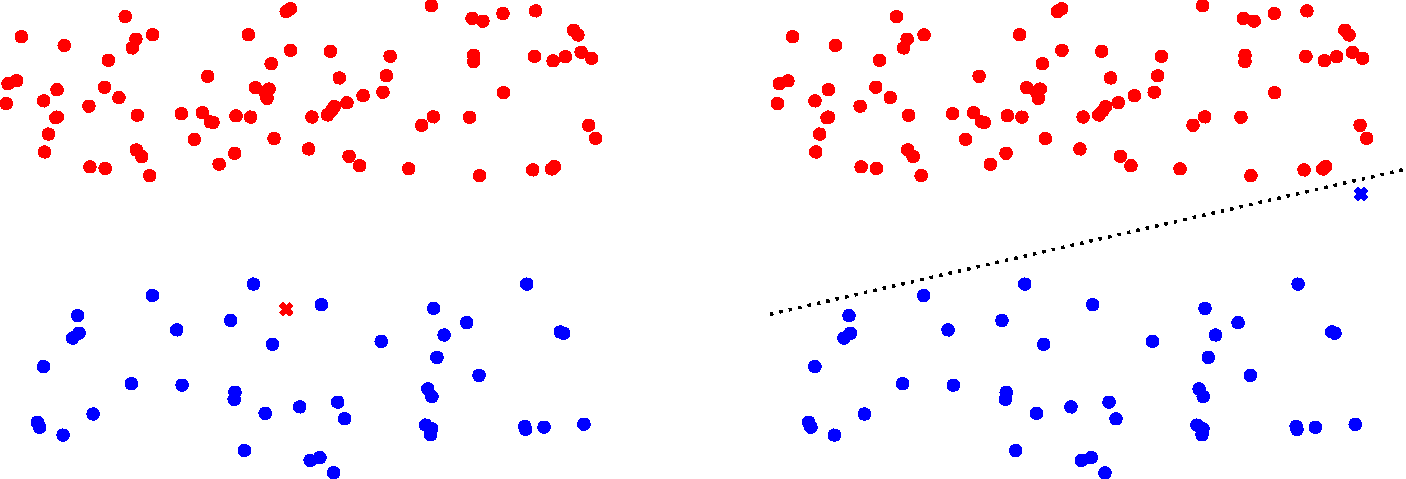
\includegraphics[width=\linewidth]{img/casi_dove_hardmargin_va_male_o_non_va.pdf}
    \caption{A sinistra un esempio di dataset non linearmente separabile, non risolvibile con il modello \emph{hard margin}. A destra un caso linearmente separabile la cui soluzione \emph{hard margin} è fortemente influenzata da un \emph{outlier}. I dati con segno ``X'' sono erroneamente etichettati.}
    \label{fig:svc:softmargin:casi_che_hardmargin_non_risolve}
\end{figure}
Per generalizzare il modello \emph{support vector classifier} e renderlo tollerante ad errori di classificazione, si riformula il problema di ottimizzazione in~\Cref{eq:svc:hardmargin:primal}, introducendo $m$ variabili di \emph{slack}/scarto $\xi_i \geq 0 \quad i=1,...,m$, una per ogni dato di addestramento. Ogni valore $\xi_i$ sarà proporzionale alla distanza tra $\Vec{x}_i$ erroneamente classificato e la superficie di separazione. $\xi_i$ sarà nulla per ogni $\Vec{x}_i$ correttamente classificato. Resta da definire come utilizzare le variabili di \emph{slack} per penalizzare la scelta di dati erroneamente classificati. 
In generale si definisce il problema primale
\begin{equation}
\begin{aligned}
& \min_{\Vec{w},b}    && \norm{\Vec{w}} + \frac{C}{p}\sum_{i=1}^{m}\xi_i^p\\
& \textrm{s.t.} && y_i(\Vec{w}\cdot\Vec{x}_i + b) \geq 1 - \xi_i, &&  i=1,\dots,m, \\
&               && \xi_i \geq 0,                 &&  i=1,\dots,m.\\
\end{aligned}
\end{equation}
Il parametro $C$, fissato a priori, determina il grado di tolleranza agli \emph{outlier}, bilanciando la funzione obiettivo originale con la penalità introdotta dalle variabili di \emph{slack}.
%
Il valore di $p$ è scelto tra $p=1$ (L1-SVC) e $p=2$ (L2-SVC). Viene qui considerata la formulazione L1-SVC:
\begin{equation}
\label{eq:svc:softmargin:primal}
\begin{aligned}
& \min_{\Vec{w},b,\Vec{\xi}}    && \norm{\Vec{w}} + C\sum_{i=1}^{m}\xi_i\\
& \textrm{s.t.} && y_i(\Vec{w}\cdot\Vec{x}_i + b) \geq 1 - \xi_i, &&  i=1,\dots,m, \\
&               && \xi_i \geq 0,                 &&  i=1,\dots,m.\\
\end{aligned}
\end{equation}
Il modello così modificato, viene chiamato \emph{soft margin support vector classifier}.
Si riporta in~\Cref{fig:soft_margin} un esempio di modello \emph{soft margin} per un insieme di dati su due dimensioni.

\begin{figure}
    \centering
    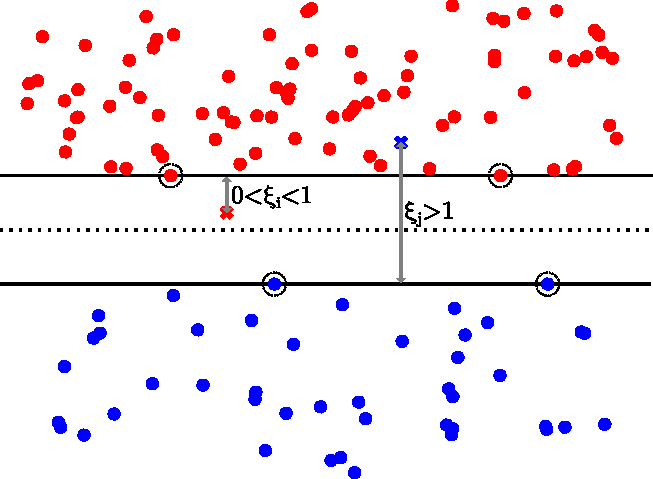
\includegraphics[width=.7\linewidth]{img/soft_margin.pdf}
    \caption{Con la formulazione \emph{soft margin} si tollerano esempi dalla parte sbagliata del margine ($\xi_i>1$) o troppo vicini al margine ($0<\xi_i<1$). I punti in questione sono rappresentati in figura con un segno ``X''.}
    \label{fig:soft_margin}
\end{figure}



\subsection{Formulazione duale}\label{subsec:soft_margin_dual}
Il procedimento per ricavare la formulazione duale è analogo al caso \emph{hard margin}.
Si riscrive la funzione obiettivo del problema~\Cref{eq:svc:softmargin:primal} e si esprimono i vincoli in forma normale, ottenendo il problema
\begin{equation}
\label{eq:svc:softmargin:primal_convenient}
\begin{aligned}
& \min_{\Vec{w},b,\Vec{\xi}}    && \frac{1}{2}\norm{\Vec{w}}^2 + C\sum_{i=1}^{m} \xi_i \\
& \textrm{s.t.} && y_i(\Vec{w}\cdot \Vec{x}_i + b) - 1 + \xi_i \geq 0, && i=1,\dots,m, \\
&               && \xi_i \geq 0,  && i=1,\dots,m.
\end{aligned}
\end{equation}
%
Si applica il metodo dei moltiplicatori di Lagrange, ottenendo la funzione lagrangiana
\begin{equation}
\label{eq:svc:softmargin:lagrange_fn}
\begin{split}
L_P(\Vec{w},b, \Vec{\xi}, \Vec{\alpha}, \Vec{\mu}) = & \frac{1}{2}\norm{\Vec{w}}^2 + C\sum_{i=1}^{m} \xi_i - \sum_{i=1}^{m} \alpha_i (y_i(\Vec{w}\cdot \Vec{x}_i +b) -1 +\xi_i) - \sum_{i=1}^{m}\mu_i\xi_i =\\
        = & \frac{1}{2}\Vec{w}\cdot\Vec{w} + C\sum_{i=1}^{m} \xi_i - \sum_{i=1}^{m} \alpha_i y_i(\Vec{w}\cdot \Vec{x}_i +b) -  \sum_{i=1}^{m} - \alpha_i  \\ & - \sum_{i=1}^{m} \alpha_i\xi_i - \sum_{i=1}^{m}\mu_i\xi_i= \\
        = & \frac{1}{2}\Vec{w}\cdot\Vec{w} + C\sum_{i=1}^{m} \xi_i - \sum_{i=1}^{m} \alpha_i y_i \Vec{w}\cdot \Vec{x}_i - b \sum_{i=1}^{m} \alpha_i y_i \\ & + \sum_{i=1}^{m} \alpha_i - \sum_{i=1}^{m} \alpha_i\xi_i - \sum_{i=1}^{m}\mu_i\xi_i,
\end{split}
\end{equation}
da minimizzare rispetto a $\Vec{w},b,\Vec{\xi}$ e da massimizzare rispetto ad $\Vec{\alpha}, \Vec{\mu}$ 
\begin{equation}
\label{eq:svc:softmargin:max_min}
\begin{aligned}
& \max_{\Vec{\alpha}, \Vec{\mu}} \min_{\Vec{w}, b, \Vec{\xi}} && L_P(\Vec{w},b, \Vec{\xi}, \Vec{\alpha}, \Vec{\mu}) \\
& \textrm{s.t.} && \alpha_i \geq 0,  && i=1,..., m,\\
&               && \mu_i \geq 0,     && i=1,..., m.\\
\end{aligned}
\end{equation}
%
Una soluzione ottima per il problema in~\Cref{eq:svc:softmargin:max_min} deve soddisfare le condizioni di Karush-Kuhn-Tucker:
\begin{align}
    \label{eq:svc:softmargin:kkt1}
    \pd{L_P(\Vec{w},b, \Vec{\xi}, \Vec{\alpha}, \Vec{\mu})}{\Vec{w}} = \Vec{0},  \\[2mm]
    \label{eq:svc:softmargin:kkt2}
    \pd{L_P(\Vec{w},b, \Vec{\xi}, \Vec{\alpha}, \Vec{\mu})}{b} = 0, \\[2mm]
    \label{eq:svc:softmargin:kkt3}
    \pd{L_P(\Vec{w},b, \Vec{\xi}, \Vec{\alpha}, \Vec{\mu})}{\Vec{\xi}} = 0, 
\end{align}
\begin{align}
    \label{eq:svc:softmargin:kkt4}
    \alpha_i^*(y_i(\Vec{x}_i\cdot\Vec{w}^*+b^*)-1+\xi_i^*) = 0,  && i=1,\dots,m, \\[2mm] 
    \label{eq:svc:softmargin:kkt5}
    \mu_i^*\xi_i^* = 0, && i=1,\dots,m, \\[2mm] 
    \label{eq:svc:softmargin:kkt6}
    \alpha_i \geq 0, \mu_i \geq 0, \xi_i \geq 0, && i=1,\dots,m.
\end{align}
Le condizioni nelle~\Cref{eq:svc:softmargin:kkt1,eq:svc:softmargin:kkt2,eq:svc:softmargin:kkt3}, ovvero
\begin{equation*}
    \begin{split}
        \pd{L}{\Vec{w}} & = \Vec{w} - \sum_{i=1}^{m}\alpha_iy_i\Vec{x}_i = \Vec{0},\\
        \pd{L}{b} &=  \sum_{i=1}^{m}\alpha_iy_i = 0,\\
        \pd{L}{\Vec{\xi}} &= C -\sum_{i=1}^{m}\alpha_i - \sum_{i=1}^{m}\mu_i = 0,
    \end{split}
\end{equation*}
si riducono a
\begin{align} 
    \label{eq:svc_hard_sub1}
    \Vec{w} = \sum_{i=1}^{m}\alpha_iy_i\Vec{x}_i,  \\[2mm]
    \label{eq:svc_hard_sub2}
    \sum_{i=1}^{m}\alpha_iy_i = 0, \\[2mm]
    \label{eq:svc_hard_sub3}
    C = \sum_{i=1}^{m}\alpha_i + \sum_{i=1}^{m}\mu_i.
\end{align}
Sostituendo le~\Cref{eq:svc_hard_sub1,eq:svc_hard_sub2,eq:svc_hard_sub3} nella funzione~(\ref{eq:svc:softmargin:lagrange_fn}) si ottiene la funzione obiettivo duale
\begin{equation}
\begin{split}
L_D(\Vec{w},b, \Vec{\xi}, \Vec{\alpha}, \Vec{\mu}) = & \frac{1}{2}\Vec{w}\cdot\Vec{w} + C\sum_{i=1}^{m} \xi_i - \sum_{i=1}^{m} \alpha_i y_i \Vec{w}\cdot \Vec{x}_i - b \sum_{i=1}^{m} \alpha_i y_i \\ & + \sum_{i=1}^{m} \alpha_i - \sum_{i=1}^{m} \alpha_i\xi_i - \sum_{i=1}^{m}\mu_i\xi_i =\\
= & \frac{1}{2}\sum_{i=1}^{m}\alpha_iy_i\Vec{x}_i \cdot \sum_{i=1}^{m}\alpha_iy_i\Vec{x}_i  + \sum_{i=1}^{m}\alpha_i\xi_i + \sum_{i=1}^{m}\mu_i\xi_i \\
& - \sum_{i=1}^{m} \alpha_i y_i  \cdot \Vec{x}_i \sum_{j=1}^{m}\alpha_jy_j\Vec{x}_j + \sum_{i=1}^{m} \alpha_i - \sum_{i=1}^{m} \alpha_i\xi_i - \sum_{i=1}^{m}\mu_i\xi_i =\\
=& \frac{1}{2}\sum_{i=1}^{m}\sum_{j=1}^{m}\alpha_i\alpha_jy_iy_j\Vec{x}_i\cdot\Vec{x}_j + \sum_{i=1}^{m} \alpha_i,
\end{split}  
\end{equation}
espressa esclusivamente in funzione di $\Vec{\alpha}$.
Aggiungendo i rimanenti vincoli si ottiene la formulazione del problema duale
\begin{equation}\label{eq:svc:softmargin:wolfe_dual}
\begin{aligned}
& \max_{\vec{\alpha}}    && \sum_{i=1}^{m}\alpha_i - \frac{1}{2}\sum_{i=1}^{m}\sum_{j=1}^{m}\alpha_i\alpha_jy_iy_j\Vec{x}_i\cdot\Vec{x}_j\\
& \textrm{s.t.} && \sum_{i=1}^{m} \alpha_iy_i = 0, \\
&               && 0 \leq \alpha_i \leq C, && i=1,\dots,m. \\
\end{aligned}
\end{equation}
Come nel caso \emph{soft margin}, $\Vec{w}^*$ e $b^*$ sono ricavati dai vettori di supporto.
Si può notare come la formulazione duale \emph{hard margin} sia sostanzialmente identica alla formulazione duale \emph{soft margin}, con la differenza che in quest'ultima i moltiplicatori lagrangiani hanno un valore limitato al massimo a $C$.

% Dimitris Bertsimas, Jack Dunn, Colin Pawlowski, Ying Daisy Zhuo (2019) Robust Classification. INFORMS Journal on Optimization 1(1):2-34. https://doi.org/10.1287/ijoo.2018.0001 '' Both the primal and dual are convex quadratic optimization problems. Because the dual problem has fewer decision variables, and the majority of these variables tend to be equal to zero or the cost parameter C in the optimal solution, it is typically the problem solved in practice (Friedman et al. 2001). In addition, the dual form is ad vantageous because it allows us to do the kernel trick to learn nonlinear decision rules (Cortes and Vapnik 1995).''



\section{\emph{Kernel trick}}\label{sec:kernel_trick}
I modelli esposti fino ad ora sono dei classificatori lineari e non sono in grado di modellare relazioni più complesse.
Come anticipato nel~\Cref{sec:kernel_methods}, si può rendere il modello SVC non lineare utilizzando una funzione \emph{kernel}.

Si potrebbe pensare di elaborare i dati prima di addestrare un modello, applicando una trasformazione in grado di renderli linearmente separabili in un nuovo spazio.
Considerando per esempio i dati mostrati in~\Cref{fig:kerneltrick:non_lin_sep}, non linearmente separabili nello spazio monodimensionale originale, si potrebbe ipotizzare di applicare una trasformazione utilizzando la funzione $\Phi:\mathbb{R} \rightarrow \mathbb{R}^2,$ con $\Phi(x) = (x, x^2)$, ottenendo un nuovo insieme di dati linearmente separabili nel nuovo spazio, mostrato in~\Cref{fig:kerneltrick:visualized}. 

\begin{figure}
    \begin{subfigure}[t]{.45\textwidth}
        \centering
        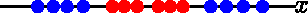
\includegraphics[width=\textwidth]{img/non_linearmente_separabili.pdf}
        \caption{Insieme di dati non linearmente separabili nello spazio originale. Il colore identifica la classe di ogni punto.}
        \label{fig:kerneltrick:non_lin_sep}
    \end{subfigure}%
    \hfill
    \begin{subfigure}[t]{.45\textwidth}
        \centering
        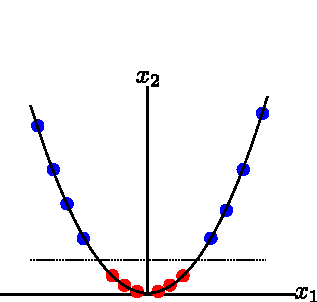
\includegraphics[width=\textwidth]{img/kernel_trick_visualized.pdf}
        \caption{I dati della~\Cref{fig:kerneltrick:non_lin_sep}, mappati nel nuovo spazio bidimensionale, sono linearmente separabili (per esempio dalla retta tratteggiata).}
        \label{fig:kerneltrick:visualized}
    \end{subfigure}%
    \caption{Esempio di trasformazione per rendere un insieme di dati linearmente separabili in un nuovo spazio.}
\end{figure}

% \begin{figure}
%     \centering
%     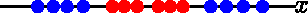
\includegraphics[width=0.5\linewidth]{img/non_linearmente_separabili.pdf}
%     \caption{Esempio in una dimensione di dati non linearmente separabili. Il colore identifica la classe di ogni punto.}
%     \label{fig:kerneltrick:non_lin_sep}
% \end{figure}
% \begin{figure}
%     \centering
%     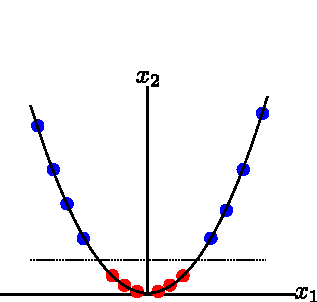
\includegraphics[width=0.5\linewidth]{img/kernel_trick_visualized.pdf}
%     \caption{I dati della~\Cref{fig:kerneltrick:non_lin_sep}, mappati nel nuovo spazio bidimensionale, sono linearmente separabili (per esempio dalla retta tratteggiata).}
%     \label{fig:kerneltrick:visualized}
% \end{figure}

In generale, si vorrebbero mappare i dati di addestramento dallo spazio originale $\mathcal{X}$ ad uno spazio delle \emph{feature} $\mathcal{H}$ di dimensioni maggiori, potenzialmente infinite, usando una funzione
\begin{equation}
\label{eq:generic_kernel_mapping}
\Phi(x_i) : \mathcal{X} \rightarrow \mathcal{H}
\end{equation}
in modo da rendere i dati linearmente separabili in $\mathcal{H}$.


Rifacendosi alla formulazione del problema \emph{soft margin} in~\Cref{eq:svc:softmargin:wolfe_dual} è possibile notare come i dati di addestramento compaiano nella funzione obiettivo esclusivamente come prodotto scalare tra di essi. 
Per applicare esplicitamente la trasformazione $\Phi$, si dovrebbe dunque calcolare $\Phi(\Vec{x}_i)\cdot\Phi(\Vec{x}_j)$ per $i=1,\dots,m$, il che renderebbe la procedura costosa dal punto di vista computazionale, se non impossibile ($\mathcal{H}$ di infinite dimensioni). 
Come anticipato nel~\Cref{sec:kernel_methods}, è possibile esprimere il prodotto scalare tra elementi appartenenti ad $\mathcal{H}$ con una funzione espressa in termini di prodotto scalare tra elementi di $\mathcal{X}$. 
Esiste la funzione \emph{kernel}
\begin{equation*}
    K: \mathcal{X} \times \mathcal{X} \rightarrow \mathbb{R} 
\end{equation*}
per cui per ogni $\Vec{x}_i, \Vec{x}_j \in \mathcal{X}$ vale
\begin{equation*}
    K(\Vec{x}_i, \Vec{x}_j) = \Phi(\Vec{x}_i) \cdot \Phi(\Vec{x}_j).
\end{equation*}
Il \emph{kernel trick} consiste nell'utilizzare una funzione \emph{kernel} $K$ in modo che la funzione $\Phi$ non debba essere calcolata esplicitamente. 
La funzione $K$, utilizzando i dati nello spazio originale, calcola un risultato equivalente al prodotto scalare tra i punti trasformati. 
Il valore $K(\Vec{x}_i, \Vec{x}_j)$ può essere interpretato come una misura della ``vicinanza'', o meglio come una una misura di similarità, tra i punti $\Vec{x}_i, \Vec{x}_j$.
Esistono diverse funzioni \emph{kernel}; le più utilizzate sono riportate nell'elenco seguente:
\begin{itemize}
    \item Kernel lineare, calcolato come
    \begin{equation*}
        K(\Vec{x}_1, \Vec{x}_2) = \Vec{x}_1\cdot\Vec{x}_2.
    \end{equation*} 
    Questo \emph{kernel} è in realtà fittizio perché la $\Phi$ corrispondente equivale all'identità $\Phi(\Vec{x}_i)=\Vec{x}_i$. Utilizzare il \emph{kernel} lineare produce un modello lineare nello spazio originale.
    \item Kernel polinomiale, calcolato come
    \begin{equation*}
        K(\Vec{x}_1, \Vec{x}_2) = (\Vec{x}_1\cdot\Vec{x}_2 + 1)^d.
    \end{equation*} 
    Questo \emph{kernel} trasforma i vettori in uno spazio a dimensione finita. L'iperparametro $d$ viene fissato a priori. Utilizzando questo \emph{kernel}, l'iperpiano di separazione nello spazio delle \emph{feature} induce una superficie di separazione nello spazio originale che corrisponde ad una superficie polinomiale di grado al massimo uguale a $d$.
    \item Kernel gaussiano, calcolato come:
    \begin{equation*}
        K(\Vec{x}_1, \Vec{x}_2) = \mathrm{exp}({-\frac{\norm{\Vec{x}_1 - \Vec{x}_2}^2}{2 \sigma^2}}).
    \end{equation*} 
    Questo \emph{kernel} trasforma i vettori in uno spazio di dimensione infinita. L'iperparametro $\sigma$ viene fissato a priori. Utilizzando questo \emph{kernel}, l'iperpiano di separazione nello spazio delle \emph{feature} induce una superficie di separazione nello spazio originale che corrisponde ad una somma di distribuzioni gaussiane multivariate con deviazione standard $\sigma$.
\end{itemize}
%
In generale, le condizioni per far sì che una funzione $K$ sia un \emph{kernel}, derivano da un noto teorema di Mercer\cite{mercer_theorem, RKHS}. Se la funzione \emph{kernel} $K$ è simmetrica, continua e definita semi-positiva, allora esiste una funzione 
\begin{equation}
    \Phi(x) : \mathbb{R}^p \rightarrow \mathcal{H}
\end{equation} 
tale per cui 
\begin{equation*}
    K(\Vec{x}_i, \Vec{x}_j) = \Phi(\Vec{x}_i)\cdot\Phi(\Vec{x}_j).
\end{equation*} 
L'introduzione del \emph{kernel trick} modifica il problema in~\Cref{eq:svc:softmargin:wolfe_dual}, che diventa quindi
\begin{equation}\label{eq:svc:softmargin:wolfe_dual_plus_kernel_trick}
\begin{aligned}
& \max_{\vec{\alpha}}    && \sum_{i=1}^{m}\alpha_i - \frac{1}{2}\sum_{i=1}^{m}\sum_{j=1}^{m}\alpha_i\alpha_jy_iy_jK(\Vec{x}_i, \Vec{x}_j)\\
& \textrm{s.t.} && \sum_{i=1}^{m} \alpha_iy_i = 0, \\
&               && 0 \leq \alpha_i \leq C, && i=1,\dots,m. \\
\end{aligned}
\end{equation}
%
La predizione della classe di un nuovo esempio $\Vec{x}_\text{test}$ sarà ottenuta calcolando 
\begin{align*}
h(\Vec{x}_\text{test})  &= \sign(\Vec{w}^*\cdot\Phi(\vec{x}_{text}) +b^*) =\\
                        &= \sign\left(\sum_{i\in S} \alpha_i^*y_i \Phi(\vec{x}_i) \cdot \Phi(\vec{x}_{text}) + b^*\right)=\\
                        &= \sign\left(\sum_{i \in S}\alpha_i^*y_iK(\Vec{x}_i, \Vec{x}_\text{test}) + b^*\right)
\end{align*}

In uno spazio con più dimensioni rispetto all'originale, è sempre possibile trovare un margine di separazione in grado di dividere i dati delle due classi perfettamente. % sempre anche con una sola dimensione in più. e.g. phi([x1]) -> [x1,y1] dove y1 è il label.
Pur essendo un risultato più preciso dal punto di vista del problema di ottimizzazione, potrebbe invece essere \emph{overfitting}. Rimane dunque cruciale la scelta del parametro $C$. 
Per valori di $C$ troppo alti, il modello cercherà di adattarsi troppo fedelmente ai dati di addestramento, creando una superficie di separazione inutilmente complessa nello spazio originale e con pessime capacità di generalizzazione. 
Al contrario, un valore basso di $C$ porterà ad una superficie di separazione più semplice e regolare, bilanciando però con più errori di classificazione. 
Per trovare un valore di $C$ soddisfacente, raggiungendo un buon compromesso tra complessità della superficie di separazione ed errori di classificazione, si utilizzano in genere delle tecniche di \emph{model selection} (viste nel~\Cref{sec:model_selection}).  


\section{Limitazioni}\label{sec:svc_limiti}
I \emph{support vector classifier} presentano alcune limitazioni di cui serve tener conto. 
Sono modelli suscettibili alla presenza di \emph{outlier}, intesi come dati erroneamente classificati o rumore. L'approccio \emph{soft-margin} consente di trattare anche problemi di questo tipo, ma la soluzione trovata potrebbe comunque subire (in misura variabile) l'effetto degli \emph{outlier}, dato che ognuno di questi punti diventerà un vettore di supporto con una relativa variabile di \emph{slack} che influirà sul valore della funzione obiettivo. 
Di conseguenza, i modelli SVC addestrati su dataset con rumore hanno in genere performance peggiori rispetto ad altri tipi di modelli pensati specificatamente per dati con molti outlier, per esempio approcci chiamati \emph{robusti} \cite{2019_robust_classification}.
La presenza di rumore nel dataset è comunque un problema comune a tutti i modelli di apprendimento automatico e non riguarda solo \emph{support vector machine}.

Una seconda limitazione riguarda la scalabilità. La procedura di addestramento considera tutti i dati disponibili e risulta quindi troppo costosa da eseguire su grandi quantità di dati, o su dati con un alto numero di feature, pur utilizzando un algoritmo di ottimizzazione numerica efficiente, come \emph{sequential minimal optimization} \cite{SMO}.

Una terza limitazione riguarda la selezione dei parametri di addestramento: il costo $C$ e la funzione \emph{kernel}. La scelta ottimale di questi valori richiede in genere molteplici esecuzioni dell'algoritmo di addestramento, moltiplicando i tempi necessari.

Risultano motivati dunque tutti gli approcci che tentano di risolvere queste limitazioni. 

